\documentclass{scrbook}
\usepackage{graphicx} % Required for inserting images
\usepackage{tabularx} % Required for fixed width tables
\usepackage{scrlayer-scrpage} % Required for the subtitles
\usepackage{url} % Required for the URLs
\usepackage{hyperref} % Required for the URLs
\usepackage{listings} % Required for the code snippets
\usepackage{mathtools} % Required for the system of equations
\usepackage{enumitem} % Required for list styling

\usepackage{fontspec}
\setmonofont{DejaVu Sans Mono} % Overleaf has this font pre-installed

% Put the caption of the snippets at the bottom
\lstset{
	captionpos=b,
	basicstyle=\ttfamily\small,
	columns=fullflexible,
	keepspaces=true
}

% Required to center the images inside table cells
\usepackage{tabularx}
\renewcommand{\tabularxcolumn}[1]{m{#1}}
\newcolumntype{C}[1]{>{\centering\arraybackslash}m{#1}}
\newcolumntype{Y}{>{\centering\arraybackslash}X}


\title{Linked Open Data}
\subtitle{Ambient intelligence course (A.Y. 2025/2026)\\Topic taught by Prof. Floriano Scioscia}
\author{Gabriele Colapinto}
\date{\today}

\begin{document}
	
	\maketitle
	\thispagestyle{empty}
	
	{\Large\textbf{License}} \\
	{Notes from Ambient intelligence (A.Y. 2025/2026) by Gabriele Colapinto. 
		Course taught by professors Michele Ruta, Floriano Scioscia, Arnaldo Tomasino, Davide Loconte — 
		Licensed under CC BY-NC 4.0.\\
		\url{https://creativecommons.org/licenses/by-nc/4.0/}}
	
	\vspace*{\fill}
	\rule{\textwidth}{0.2pt}
	\small{© 2025 Gabriele Colapinto \\
		Released under the \href{https://creativecommons.org/licenses/by-nc/4.0/}{Creative Commons Attribution–NonCommercial 4.0 International License}}
	
	\clearpage
	
	\tableofcontents
	
	\chapter{Linked Open Data Foundations}
	
	\section{From Machine-Readable to Machine-Linkable Data}
	
	A dataset is machine-readable when software can parse its content without relying on manual interpretation. This property is necessary for automated processing, but it is not sufficient for data integration on the Web. Linked Data requires a stronger condition: data items must be identifiable, dereferenceable, and connectable to other data items through explicit semantic relations.\\
	
	The Resource Description Framework (RDF) is central to this distinction. RDF is not primarily a file format; it is a data model for representing information as statements. Each RDF statement is a triple composed of a subject, a predicate, and an object. The subject denotes the resource being described, the predicate denotes the property or relation, and the object denotes either another resource or a literal value. A set of RDF triples forms a graph, because resources can be connected by predicates to other resources.\\
	
	The same RDF graph can be exchanged through different serialization formats. The essential aspect is therefore not the concrete syntax used to write the data, but the graph-based model and the use of globally identifiable names. In the Linked Data vision, these names are Uniform Resource Identifiers (URIs). A URI is not only an internal database key: it is a Web identifier that can be shared across independently produced datasets. When a URI is used consistently, applications and third parties can recognize that different statements refer to the same resource or to related resources.\\
	
	Machine-linkable data enables interoperability at Web scale. Different organizations may publish datasets independently, using different infrastructures and publication schedules, while still making their resources connectable. Links can be created by the original publishers or by third parties. This makes it possible to build an open graph of data in which resources from distinct datasets mutually enrich each other.
	
	\section{Principles of Linked Data}
	
	Linked Data is based on a small set of publication principles. The first principle is to use URIs to name resources. A resource may be a document, a person, a place, an event, an abstract concept, a product, or any other entity that needs to be described.\\
	
	The second principle is to use dereferenceable URIs. In practice, URIs should normally rely on the HTTP protocol, so that clients can look them up using standard Web mechanisms. Looking up a URI should return a useful description of the resource. This description may be provided in RDF for machine processing, in HTML for human users, or in multiple representations through content negotiation.\\
	
	The third principle is to include links to other URIs in resource descriptions. Such links are what transform isolated RDF graphs into Linked Data. A description should not only contain local attributes, but should also connect the resource to external resources whenever meaningful. These outgoing links allow clients to discover further data and allow independent datasets to become part of a larger data space.\\
	
	These principles can be summarized as follows:
	
	\begin{itemize}
	    \item identify resources with URIs;
	    \item prefer HTTP URIs, so that resources can be looked up on the Web;
	    \item return useful descriptions when URIs are dereferenced;
	    \item use standard technologies, such as RDF and HTML, for those descriptions;
	    \item include links to other URIs, so that additional resources can be discovered.
	\end{itemize}
	
	The expression \emph{Linked Open Data} adds the openness requirement to Linked Data. Data is open when it is made available under a license that permits reuse. A dataset can be linked without being open, and it can be open without being well linked. Linked Open Data combines both aspects: legal reusability and semantic interconnection.
	
	\section{The Five-Star Model for Linked Open Data}
	
	The five-star model is a practical way to classify the maturity of open data publication. The model is cumulative: each level includes the requirements of the previous levels and adds a stronger technical condition.\\
	
	\begin{tabularx}{\linewidth}{|C{0.15\textwidth}|C{0.3\textwidth}|Y|}
		\hline
		\textbf{Level} & \textbf{Open Data rating badge} & \textbf{Requirement} \\
		\hline
		
		1 star &
		\vspace{2mm}
\includegraphics[width=\linewidth]{"Images/1_star_badge.jpg"} &
		The data is available on the Web in any format and is distributed with an open license. (OL = Open License) \\
		\hline
		
		2 stars &
		\vspace{2mm}
\includegraphics[width=\linewidth]{"Images/2_stars_badge.jpg"} &
		The data is available in a machine-readable format, for example as a spreadsheet file. (RE = REadable) \\
		\hline
		
		3 stars &
		\vspace{2mm}
\includegraphics[width=\linewidth]{"Images/3_stars_badge.jpg"} &
		The data is available in a non-proprietary machine-processable format, for example CSV. (OF = Open Format)\\
		\hline
		
		4 stars &
		\vspace{2mm}
\includegraphics[width=\linewidth]{"Images/4_stars_badge.jpg"} &
		The data is available using W3C standards, for example RDF. (URI idicates the fact that data is identified using an URI)\\
		\hline
		
		5 stars &
		\vspace{2mm}
\includegraphics[width=\linewidth]{"Images/5_stars_badge.jpg"} &
		The data satisfies the previous conditions and includes links to other open datasets. (LD = Linked Data)\\
		\hline
	\end{tabularx}
	
	The transition from the first to the third level concerns accessibility and technical independence. A dataset published as a scanned document may satisfy minimal availability, but it is costly to process automatically. A spreadsheet improves machine readability, while a non-proprietary format reduces dependence on a specific vendor.\\
	
	The fourth level introduces Web standards for semantic representation. Publishing data in RDF makes it possible to express the dataset as a graph of typed statements and to identify resources through URIs. The fifth level completes the Linked Data objective: the dataset does not remain isolated, but connects its resources to resources in other open datasets.\\
	
	This rating model is useful because it separates several dimensions that are sometimes confused. Openness depends on licensing. Machine readability depends on the technical format. Linkability depends on the use of identifiers, standard vocabularies, and explicit cross-dataset links.
	
	\section{Dataset Discovery and the Linked Open Data Cloud}
	
	\begin{figure}
		\centering
		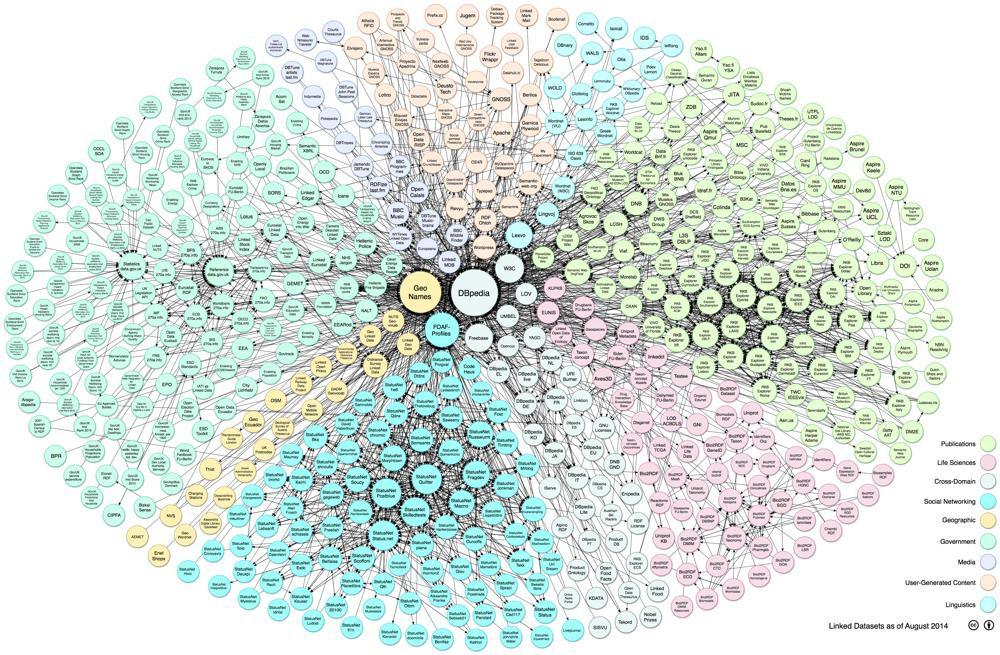
\includegraphics[width=\linewidth]{Images/Open_Data_Cloud.jpg}
		\caption{Open Data Cloud involving various domains}
		\label{fig:open_data_cloud}
	\end{figure}
	
	A Linked Open Data ecosystem requires not only publication principles, but also mechanisms for discovering datasets. Public catalogues and registries collect dataset descriptions and provide entry points for reuse. Examples include DBpedia, collections of RDF dataset dumps, general Linked Data catalogues, DataHub, and national or community catalogues such as Italian Linked Open Data portals.\\
	
	The Linked Open Data cloud is a representation of the interconnection among published datasets. It contains more than a thousand interlinked datasets organized by domain. Domains are commonly represented with different colors in cloud diagrams, while edges represent links between datasets. The visualization emphasizes that Linked Open Data is not a single centralized database, but a distributed data space maintained by many publishers.\\
	
	DBpedia is historically one of the most central datasets in this cloud (see figure \ref{fig:open_data_cloud}). Its centrality is due to the breadth of the resources extracted from Wikipedia and to the large number of external datasets that link to DBpedia identifiers. Such central datasets often function as hubs: they provide widely reused URIs for entities that many other datasets need to reference.\\
	
	The cloud perspective also clarifies why Linked Data is more than publishing RDF files. An RDF dataset that uses only local identifiers and provides no outgoing links may be machine-processable, but it contributes weakly to the larger Web of Data. A well-published dataset should expose stable identifiers, use shared vocabularies when possible, and establish links to authoritative external resources.
	
	\section{Design Implications}
	
	Publishing Linked Open Data requires design decisions at several levels. At the identification level, publishers must define URI patterns that are stable, meaningful enough for management, and independent from implementation details that may change. At the description level, they must decide which properties and vocabularies describe the resources accurately. At the interlinking level, they must identify external datasets that contain resources corresponding to the same entities or to semantically relevant related entities.\\
	
	The use of shared vocabularies is important for interoperability. When a dataset describes common notions through widely adopted terms, consumers can interpret its structure more easily and combine it with other datasets with less custom mapping. When no existing vocabulary is expressive enough, a new vocabulary may be defined, but reuse remains preferable for the parts of the model that are already covered by established terms.\\
	
	The resulting publication process can be seen as a progression from raw availability to semantic integration. Open licensing makes reuse legally possible. Machine-readable and non-proprietary formats make reuse technically feasible. RDF and URIs make resources identifiable and graph-based. Links to other datasets make the data part of a broader Web of Data.
	
	\chapter{Core Vocabularies for Linked Open Data}
	
	Linked Open Data relies not only on RDF triples and dereferenceable identifiers, but also on shared vocabularies. A vocabulary provides classes and properties whose meaning is already understood by a community of users and applications. Reusing established vocabularies improves interoperability because independently produced datasets can describe comparable entities with the same terms, and because clients can interpret those terms without learning a new ad hoc schema.\\
	
	A vocabulary should be selected according to the modeling need. Some vocabularies describe general metadata about resources, others represent people and social relations, controlled terminologies, products, services, or commercial offers. In practice, a dataset often combines several vocabularies: one may use Dublin Core for metadata, SKOS for categories, FOAF for persons, and domain-specific terms for concepts not covered by existing models.
	
	\section{SKOS: Simple Knowledge Organization System}
	
	The Simple Knowledge Organization System, usually abbreviated as \texttt{skos}, is an RDF vocabulary for representing knowledge organization systems such as thesauri, taxonomies, subject headings, classification schemes, and controlled vocabularies. It is particularly useful when the dataset needs to describe topics, categories, or concepts and their relationships, without committing to the stronger logical constraints of an OWL ontology.\\
	
	The SKOS namespace is:
	
	\begin{lstlisting}
http://www.w3.org/2004/02/skos/core#
	\end{lstlisting}
	
	and it is normally declared as follows:
	
	\begin{lstlisting}
@prefix skos: <http://www.w3.org/2004/02/skos/core#> .
	\end{lstlisting}
	
	The central class is \texttt{skos:Concept}. A SKOS concept denotes a unit of thought or a topic that can be used for classification, indexing, retrieval, or annotation. A concept is not necessarily a class in the ontological sense: it is primarily an element of a conceptual scheme. This distinction is important because a topic such as ``science fiction films'' can be used to classify works without implying that the concept itself is an RDF class whose instances are all science fiction films.
	
	\subsection{Concept Schemes and Concept Description}
	
	A concept may belong to a scheme through \texttt{skos:inScheme}. The scheme identifies the controlled vocabulary or classification system in which the concept is defined. Concept descriptions normally include labels, notes, and links to related concepts or to equivalent concepts in other datasets.\\
	
	The following example describes a concept from a news-oriented classification scheme and links it to an external resource:
	
	\begin{lstlisting}
@prefix nyt:  <http://data.nytimes.com/elements/> .
@prefix skos: <http://www.w3.org/2004/02/skos/core#> .
	
<http://data.nytimes.com/48662871776634757120>
  a skos:Concept ;
  skos:inScheme nyt:nytd_des ;
  skos:narrowMatch <http://dbpedia.org/resource/Ethics> ;
  skos:prefLabel "Ethics"@en ;
  skos:scopeNote "Used for issues of morality but also for unethical
  behavior..."@en .
	\end{lstlisting}
	
	The language tag in a literal, as in \texttt{"Ethics"@en}, specifies the language of the lexical form. This makes multilingual vocabularies possible without creating separate properties for each language.
	
	\subsection{Labels}
	
	SKOS distinguishes among different kinds of labels. The distinction is useful for search, indexing, and user interfaces.
	
	\begin{itemize}
	    \item \texttt{skos:prefLabel} is the preferred lexical form used to display or refer to a concept. A concept should have at most one preferred label per language.
	    \item \texttt{skos:altLabel} represents alternative lexical forms, such as synonyms, abbreviations, spelling variants, or common names.
	    \item \texttt{skos:hiddenLabel} represents labels that should not be displayed to users but may be useful internally, for example to support search over frequent misspellings.
	\end{itemize}
	
	These properties are subproperties of \texttt{rdfs:label}:
	
	\begin{lstlisting}
skos:prefLabel   rdfs:subPropertyOf rdfs:label .
skos:altLabel    rdfs:subPropertyOf rdfs:label .
skos:hiddenLabel rdfs:subPropertyOf rdfs:label .
	\end{lstlisting}
	
	This design allows generic RDF tools that understand \texttt{rdfs:label} to still retrieve labels, while SKOS-aware tools can exploit the more precise distinction between preferred, alternative, and hidden forms.
	
	\subsection{Semantic Relations Between Concepts}
	
	SKOS provides properties for relating concepts within or across schemes. The main hierarchical properties are \texttt{skos:broader} and \texttt{skos:narrower}. The former links a concept to a more general concept, while the latter links a concept to a more specific one. These relations are useful for navigation, query expansion, and classification.\\
	
	Although \texttt{skos:broader} resembles \texttt{rdfs:subClassOf} at an intuitive level, the two properties have different semantics. \texttt{rdfs:subClassOf} states a class-inclusion relation between classes, whereas \texttt{skos:broader} relates concepts inside a knowledge organization system. A SKOS hierarchy is therefore a conceptual hierarchy, not necessarily a formal ontology of classes.\\
	
	The property \texttt{skos:related} expresses an associative relation between concepts. It is symmetric: if concept \(A\) is related to concept \(B\), then \(B\) is also related to \(A\). This relation is appropriate when two concepts are semantically connected but neither is a broader or narrower specialization of the other.\\
	
	SKOS also includes mapping properties to relate concepts across different schemes. For example, \texttt{skos:closeMatch} indicates a high degree of similarity without asserting strict identity, while \texttt{skos:exactMatch} is used when two concepts can be treated as equivalent for many applications.
	
	\subsection{Example: Subject Headings}
	
	The following example represents a subject heading as a SKOS concept and connects it to broader, narrower, and externally matched concepts:
	
	\begin{lstlisting}
@prefix skos: <http://www.w3.org/2004/02/skos/core#> .
	
<http://id.loc.gov/authorities/subjects/sh85118660>
  a skos:Concept ;
  skos:prefLabel "Science fiction films"@en ;
  skos:broader <http://id.loc.gov/authorities/subjects/sh85088084> ;
  skos:closeMatch <http://d-nb.info/gnd/4054023-6> ;
  skos:exactMatch <http://stitch.cs.vu.nl/vocabularies/rameau/ark:/12148/cb11931406w> ;
  skos:example "Note under [Science fiction]" ;
  skos:inScheme <http://id.loc.gov/authorities/subjects> ;
  skos:narrower
      <http://id.loc.gov/authorities/subjects/sh85127380>,
      <http://id.loc.gov/authorities/subjects/sh85127382> .
	\end{lstlisting}
	
	The example shows two typical uses of SKOS in Linked Data. Internally, it organizes concepts inside a scheme through broader and narrower relations. Externally, it connects one scheme to other datasets through match relations. Dereferencing the linked URIs allows applications to discover additional descriptions and to expand navigation or search across dataset boundaries.
	
	\section{Dublin Core Metadata}
	
	Dublin Core is a general metadata vocabulary originally designed to describe textual resources, but it is now widely used for many kinds of digital and physical resources. It is useful when a dataset needs concise, interoperable descriptions of resources such as documents, datasets, images, records, publications, or web pages.\\
	
	The original Dublin Core Metadata Element Set contains fifteen main properties. The namespace of the element set is:
	
	\begin{lstlisting}
http://purl.org/dc/elements/1.1/
	\end{lstlisting}
	
	Common prefixes are \texttt{dc} and \texttt{dcterms}. In current RDF datasets, \texttt{dcterms} is often preferred because it belongs to the broader DCMI (Dublin Core Metadata Initiative) Metadata Terms specification.
	
	\subsection{Main Metadata Properties}
	
	The fifteen core properties cover the most common descriptive needs:
	
	\begin{itemize}
	    \item \texttt{dc:title}: the name assigned to the resource.
	    \item \texttt{dc:creator}: the entity primarily responsible for producing the content.
	    \item \texttt{dc:subject}: the main topic of the resource.
	    \item \texttt{dc:description}: a description of the content.
	    \item \texttt{dc:publisher}: the entity responsible for publishing the resource.
	    \item \texttt{dc:contributor}: an entity that contributed to the content but is not the primary creator.
	    \item \texttt{dc:date}: a date associated with an event in the life cycle of the resource.
	    \item \texttt{dc:type}: the nature or genre of the resource.
	    \item \texttt{dc:format}: the physical or digital manifestation of the resource.
	    \item \texttt{dc:identifier}: a unique reference to the resource within a given context.
	    \item \texttt{dc:source}: a resource from which the described resource is derived.
	    \item \texttt{dc:language}: the language of the intellectual content.
	    \item \texttt{dc:relation}: a related resource.
	    \item \texttt{dc:coverage}: the spatial, temporal, or thematic scope of the resource.
	    \item \texttt{dc:rights}: information about rights, licensing, or access conditions.
	\end{itemize}
	
	The meaning of each property is intentionally broad. This makes Dublin Core suitable for lightweight metadata, but it also requires care when precise semantics are needed. For example, \texttt{dc:relation} can express a generic relation to another resource, whereas a more specific vocabulary should be preferred when the nature of the relation is important.\\
	
	A compact Dublin Core description may combine literal values and resource links:
	
	\begin{lstlisting}
@prefix dc: <http://purl.org/dc/elements/1.1/> .
	
<http://example.org/book/123>
  dc:title "Example Book"@en ;
  dc:creator <http://example.org/person/alice> ;
  dc:subject <http://example.org/concept/linked-data> ;
  dc:language "en" ;
  dc:source <http://example.org/book/original> ;
  dc:rights <http://creativecommons.org/licenses/by/4.0/> .
	\end{lstlisting}
	
	The property \texttt{dc:source} is particularly useful for derivative resources, such as translations or adaptations, because it links the described resource to the resource from which it was derived. The property \texttt{dc:coverage} is useful when a resource covers a temporal interval, a geographical area, or a specific scope, for example an archival volume that collects issues of a periodical published during a given time span.
	
	\section{FOAF: Friend of a Friend}
	
	FOAF is an ontological vocabulary for representing people, their contact information, and their relations with other people, organizations, and web resources. It is one of the earliest widely adopted Semantic Web vocabularies and remains relevant as a simple model for personal profiles and social links.\\
	
	The FOAF namespace is:
	
	\begin{lstlisting}
http://xmlns.com/foaf/0.1/
	\end{lstlisting}
	
	and is normally declared with the prefix \texttt{foaf}.\\
	
	The basic class is \texttt{foaf:Person}. A person can be described with properties such as \texttt{foaf:name}, \texttt{foaf:givenname}, \texttt{foaf:family\_name}, \texttt{foaf:title}, \texttt{foaf:gender}, \texttt{foaf:homepage}, and \texttt{foaf:weblog}. Email addresses may be represented through \texttt{foaf:mbox}, while \texttt{foaf:mbox\_sha1sum} can be used to publish a hash rather than the mailbox URI itself. Relations between people can be represented with \texttt{foaf:knows}.\\
	
	The following example describes two people and a relation between them:
	
	\begin{lstlisting}
@prefix foaf:     <http://xmlns.com/foaf/0.1/> .
@prefix matrix101: <http://thematrix101.com/#> .
	
matrix101:thomas.anderson
  a foaf:Person ;
  foaf:mbox <mailto:Thomas.Anderson@thematrix101.com> ;
  foaf:mbox_sha1sum "40398966717b6bd54fdb1304137b145878f97526" ;
  foaf:name "Thomas A. Anderson" ;
  foaf:gender "Male" ;
  foaf:title "Mr" ;
  foaf:givenname "Thomas A." ;
  foaf:family_name "Anderson" ;
  foaf:homepage <http://www.thematrix101.com/neo/> ;
  foaf:weblog <http://www.thematrix101.com/neo/blog/> .
	
matrix101:neo foaf:knows matrix101:trinity .
	
matrix101:trinity
  a foaf:Person ;
  foaf:name "Trinity" .
	\end{lstlisting}
	
	FOAF is intentionally lightweight. It is suitable for publishing basic information about agents and relationships, but specialized domains often require additional vocabularies. For example, organizational roles, employment contracts, authentication data, and privacy-sensitive profile attributes should be modeled with more appropriate domain vocabularies or application-specific extensions.
	
	\section{GoodRelations}
	
	GoodRelations is a vocabulary for describing commercial scenarios, especially products, services, offerings, prices, quantities, and business entities. It is designed to support e-commerce and marketplace data, but the same modeling pattern can be applied more generally to commerce-related resources.\\
	
	The GoodRelations namespace is:
	
	\begin{lstlisting}
http://purl.org/goodrelations/v1#
	\end{lstlisting}
	
	and is usually declared with the prefix \texttt{gr}.
	
	\subsection{Main Entities}
	
	GoodRelations organizes commercial descriptions around four main kinds of entities:
	
	\begin{itemize}
	    \item \texttt{gr:BusinessEntity}: an agent involved in commercial activity, such as a person, company, or organization.
	    \item \texttt{gr:ProductOrService}: the object of a commercial transaction, such as a product, service, or product category.
	    \item \texttt{gr:Offering}: a concrete commercial promise, including the business function, price, availability, and object offered.
	    \item \texttt{gr:Location}: a location associated with a business entity or an offer.
	\end{itemize}
	
	A key modeling distinction is between an abstract product or service category and a concrete instance being offered. For concrete items, GoodRelations provides classes such as\\
	\texttt{gr:ActualProductOrServiceInstance}. Quantitative attributes can be represented as resources, for example with \texttt{gr:QuantitativeValueFloat}, so that values and units of measurement are explicit.
	
	\newpage
	\subsection{Business Entity and Product Description}
	
	The following example defines a business entity and a monitor offered by that entity. A domain-specific namespace is used for computer-related classes and properties, while GoodRelations provides the commerce-oriented structure.
	
	\begin{lstlisting}
@prefix gr:       <http://purl.org/goodrelations/v1#> .
@prefix xsd:      <http://www.w3.org/2001/XMLSchema#> .
@prefix computer: <http://ontology/example/computer#> .
@prefix rdfs:     <http://www.w3.org/2000/01/rdf-schema#> .
	
computer:ComputerCom
  a gr:BusinessEntity ;
  rdfs:seeAlso <http://www.computer.com> ;
  gr:legalName "Computer.com"^^xsd:string .
	
computer:LG2000Monitor
  a computer:Monitor, gr:ActualProductOrServiceInstance ;
  computer:hasScreenSize computer:Size .
	
computer:Size
  a gr:QuantitativeValueFloat ;
  gr:hasUnitOfMeasurement "CMT"^^xsd:string ;
  gr:hasValueFloat "32.0"^^xsd:float .
	\end{lstlisting}
	
	The monitor is typed both as a domain-specific \texttt{computer:Monitor} and as a GoodRelations product or service instance. This combination is typical in Linked Data: a general-purpose vocabulary provides a shared commercial model, while a domain vocabulary expresses more specific characteristics.
	
	\subsection{Offering, Price, and Quantity}
	
	An offering connects the business entity to the commercial conditions under which a product or service is made available. The business function specifies whether the offer is for selling, renting, repairing, or another commercial activity. Price and quantity are modeled as separate resources so that currency, numeric value, unit, and referenced good can be described explicitly.
	
	\begin{lstlisting}
@prefix gr:       <http://purl.org/goodrelations/v1#> .
@prefix xsd:      <http://www.w3.org/2001/XMLSchema#> .
@prefix computer: <http://ontology/example/computer#> .
	
computer:Offer_1
  a gr:Offering ;
  gr:hasBusinessFunction gr:Sell ;
  gr:hasPriceSpecification computer:Price ;
  gr:includesObject computer:Quantity .

computer:Price
  a gr:UnitPriceSpecification ;
  gr:hasCurrency "EUR"^^xsd:string ;
  gr:hasCurrencyValue "200.0"^^xsd:float ;
  gr:hasUnitOfMeasurement "C62"^^xsd:string .

computer:Quantity
  a gr:TypeAndQuantityNode ;
  gr:amountOfThisGood "1.0"^^xsd:float ;
  gr:hasUnitOfMeasurement "C62"^^xsd:string ;
  gr:typeOfGood computer:LG2000Monitor .
	
computer:ComputerCom
  gr:offers computer:Offer_1 .
	\end{lstlisting}
	
	The resource \texttt{computer:Offer\_1} is the concrete offer. It states that the business function is \texttt{gr:Sell}, that the price is expressed in euros with value \texttt{200.0}, and that the offer includes one unit of the monitor. The link \texttt{gr:offers} associates the business entity with the offering.\\
	
	GoodRelations can represent more detailed commercial data than this minimal example, including richer product classifications, conditions, quantities, and locations. Its main contribution is the separation between the seller, the offered object, and the offer itself. This separation avoids conflating a product description with a temporary commercial condition such as a price or availability.
	
	\section{Combining Vocabularies}
	
	Real Linked Data descriptions frequently combine vocabularies instead of relying on a single schema. A resource can be annotated with Dublin Core metadata, classified with SKOS concepts, related to people through FOAF, and described commercially with GoodRelations. The RDF data model supports this combination because each property and class is identified by its own URI.\\
	
	The following small fragment illustrates this style of modeling:
	
	\begin{lstlisting}
@prefix dc:   <http://purl.org/dc/elements/1.1/> .
@prefix skos: <http://www.w3.org/2004/02/skos/core#> .
@prefix foaf: <http://xmlns.com/foaf/0.1/> .
@prefix ex:   <http://example.org/> .
	
ex:dataset42
  dc:title "Catalogue of Digital Publications"@en ;
  dc:creator ex:alice ;
  dc:subject ex:concept/digital-libraries .
	
ex:alice
  a foaf:Person ;
  foaf:name "Alice Rossi" .
	
ex:concept/digital-libraries
  a skos:Concept ;
  skos:prefLabel "Digital libraries"@en ;
  skos:broader ex:concept/libraries .
	\end{lstlisting}
	
	This modularity is central to Linked Open Data engineering. Existing vocabularies should be reused whenever they capture the intended meaning with sufficient precision. New classes and properties should be introduced only for domain aspects that cannot be adequately expressed with existing terms. Partial reuse is still valuable: adopting a shared vocabulary for the parts it models well reduces ambiguity and makes the dataset easier to integrate with other sources.
	
	\chapter{DBpedia and Linked Data Reuse}
	
	DBpedia is one of the canonical datasets of the Linked Open Data ecosystem. It exposes structured knowledge extracted from Wikipedia as RDF, using dereferenceable URIs, shared vocabularies, multilingual descriptions, and explicit links between resources. Its importance is not only quantitative. DBpedia is frequently used as a hub dataset because many independently produced datasets can link their entities to DBpedia resources and thereby obtain a common reference point.\\
	
	The central idea is to transform semi-structured information already present in Wikipedia into machine-linkable data. Wikipedia articles contain natural-language text, but many of them also contain infoboxes, categories, language links, and structured templates. DBpedia exploits these elements to produce RDF descriptions that can be queried, linked, and reused by applications.
	
	\section{DBpedia as a Semantic Web Version of Wikipedia}
	
	DBpedia can be understood as a Semantic Web representation of Wikipedia. Each relevant Wikipedia page is associated with a DBpedia resource, and the structured information available in the page is converted into RDF statements. In this conversion, an article topic becomes the subject of triples, infobox fields become predicates or are mapped to ontology properties, and infobox values become objects.\\
	
	For example, an infobox describing a film can be converted into triples in which the film is the subject, properties such as director, release date, genre, or starring actor are predicates, and the corresponding values are resources or literals. The important change is that values are no longer only strings displayed inside an HTML page: whenever possible, they become references to other RDF resources.\\
	
	A simplified representation of this idea is shown below:
	
	\begin{lstlisting}
@prefix dbr: <http://dbpedia.org/resource/> .
@prefix dbo: <http://dbpedia.org/ontology/> .
@prefix xsd: <http://www.w3.org/2001/XMLSchema#> .

dbr:The_Matrix
  a dbo:Film ;
  dbo:director dbr:The_Wachowskis ;
  dbo:starring dbr:Keanu_Reeves ;
  dbo:releaseDate "1999-03-31"^^xsd:date .
	\end{lstlisting}
	
	The example illustrates the extraction principle rather than the full complexity of the DBpedia dataset. The resource \texttt{dbr:The\_Matrix} is described as a film and is connected to other resources such as the directors and actors. These links are what make the dataset useful in the Linked Data sense: the description of a film can be expanded by dereferencing the URIs of related people, works, places, categories, and other entities.
	
	\section{Resource URIs}
	
	DBpedia resource identifiers are systematically derived from Wikipedia article URLs. For an English Wikipedia page such as:
	
	\begin{lstlisting}
http://en.wikipedia.org/wiki/The_Matrix
	\end{lstlisting}
	
	the corresponding DBpedia resource URI is:
	
	\begin{lstlisting}
http://dbpedia.org/resource/The_Matrix
	\end{lstlisting}
	
	This rule gives DBpedia a predictable naming scheme. The article title becomes the local part of the DBpedia resource URI, while the \texttt{http://dbpedia.org/resource/} namespace identifies the DBpedia resource space. In Turtle examples, this namespace is commonly abbreviated with the prefix \texttt{dbr}:
	
	\begin{lstlisting}
@prefix dbr: <http://dbpedia.org/resource/> .
dbr:The_Matrix
	\end{lstlisting}
	
	A predictable URI policy is useful for both publishers and consumers. Publishers can create links to DBpedia resources without manually inventing identifiers, and consumers can recognize that many datasets are referring to the same well-known entity. This is especially relevant for entity reconciliation, where local identifiers from different systems must be aligned with a shared Web identifier.\\
	
	Dereferenceability remains essential. A DBpedia URI is not merely a symbolic name: looking it up should return a useful description of the resource, in a representation suitable for human or machine consumption. This aligns DBpedia with the Linked Data principles introduced earlier: name things with URIs, make those URIs dereferenceable, and include links to other URIs in the returned descriptions.
	
	\section{From Infoboxes to RDF}
	
	\begin{figure}
		\centering
		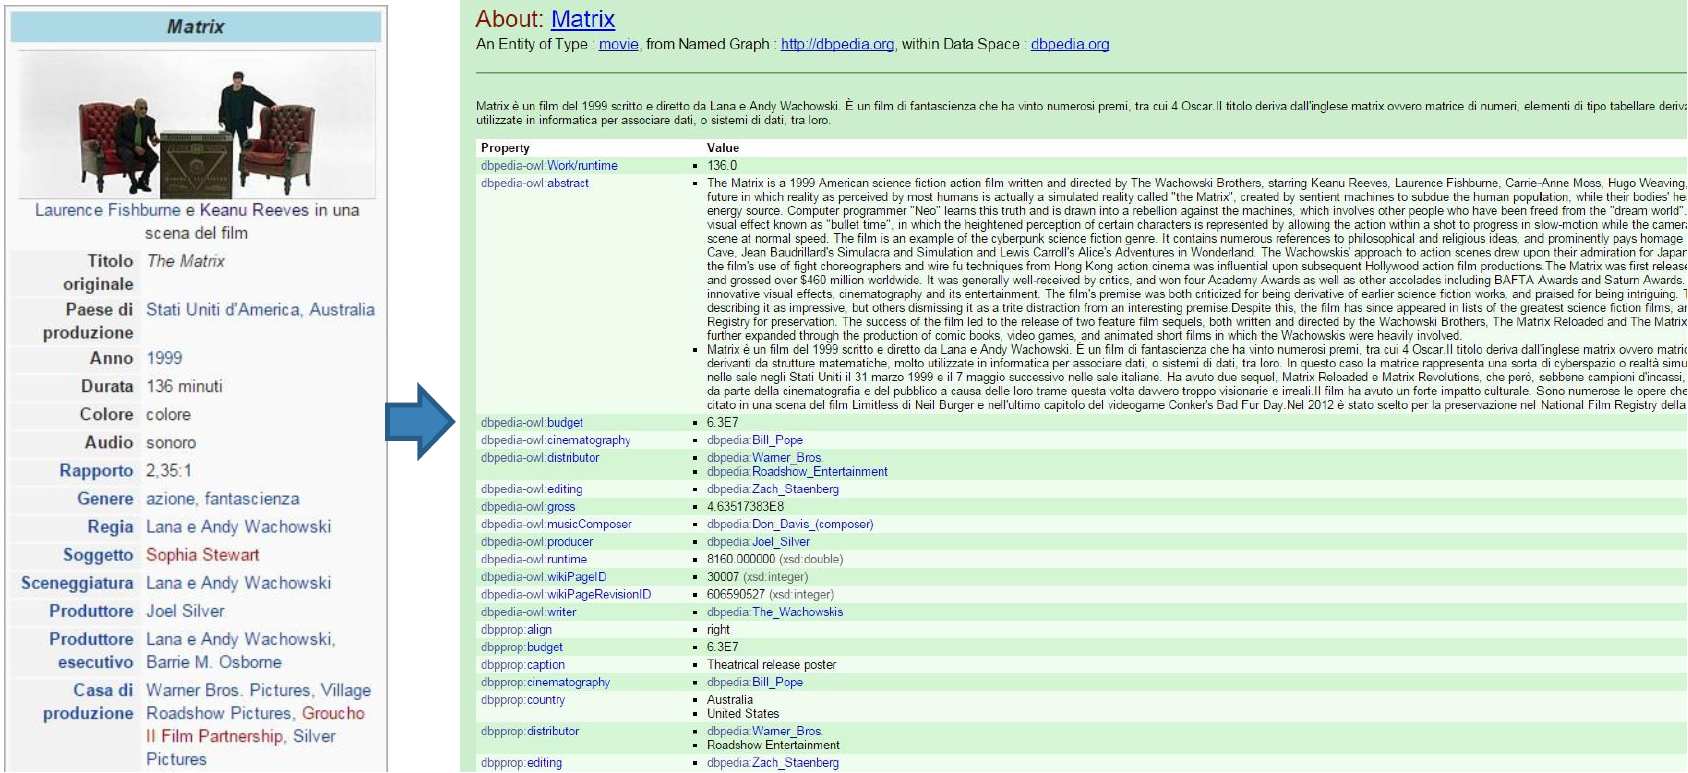
\includegraphics[width=\linewidth]{Images/Infobox_to_RDF.png}
		\caption{Infobox to RDF conversion}
		\label{fig:infobox_to_rdf}
	\end{figure}
	
	The extraction of RDF from Wikipedia relies heavily on infoboxes (see figure \ref{fig:infobox_to_rdf}). An infobox is a structured summary associated with an article, usually displayed as a table of attribute--value pairs. Since the page title identifies the described entity and the fields identify properties, the infobox can be transformed naturally into RDF triples.\\
	
	At the simplest level, a field can be translated directly:
	
	\begin{lstlisting}
Subject:   dbr:The_Matrix
Predicate: dbp:director
Object:    dbr:The_Wachowskis
	\end{lstlisting}
	
	In RDF/Turtle syntax, the same statement can be written as:
	
	\begin{lstlisting}
@prefix dbr: <http://dbpedia.org/resource/> .
@prefix dbp: <http://dbpedia.org/property/> .
dbr:The_Matrix dbp:director dbr:The_Wachowskis .
	\end{lstlisting}
	
	This direct translation is useful but not always sufficient. Wikipedia infoboxes are created by a large community and may contain heterogeneous field names, different conventions across languages, and values that require normalization. For this reason, DBpedia distinguishes between raw or template-derived properties and mappings to a more coherent ontology.
	
	\subsection{Ontology-Based Extraction}
	
	The DBpedia Ontology is an OWL ontology developed manually to provide a stable conceptual model for the extracted data. It mirrors recurring information patterns found in Wikipedia infoboxes, but it does not simply reproduce every template field as an independent property. Instead, it defines classes and properties that can be reused consistently across resources.\\
	
	For instance, many pages describe persons, places, organizations, creative works, events, or products. The ontology provides classes such as \texttt{dbo:Person}, \texttt{dbo:Place}, \texttt{dbo:Organisation}, and \texttt{dbo:Work}, together with properties suitable for those classes. Mapping infobox fields to ontology properties reduces ambiguity and makes queries more robust.\\
	
	The difference between a raw property and an ontology property can be illustrated as follows:
	
	\begin{lstlisting}
@prefix dbr: <http://dbpedia.org/resource/> .
@prefix dbp: <http://dbpedia.org/property/> .
@prefix dbo: <http://dbpedia.org/ontology/> .

dbr:The_Matrix dbp:director dbr:The_Wachowskis .
dbr:The_Matrix dbo:director dbr:The_Wachowskis .
	\end{lstlisting}
	
	The first predicate belongs to the \texttt{dbp} namespace and corresponds more closely to the extracted property name. The second predicate belongs to the \texttt{dbo} namespace and represents the mapped ontology-level relation. When available, ontology properties are generally preferable for data integration because their intended meaning is more controlled.
	
	\subsection{Literals, Resources, and Normalization}
	
	Infobox values may become literals or resources. Numeric values, dates, textual descriptions, and measurements may be represented as typed literals. Values that denote entities should preferably become URIs. This distinction matters because literals terminate the graph, while URIs allow further navigation.\\
	
	Consider the following simplified example:
	
	\begin{lstlisting}
@prefix dbr: <http://dbpedia.org/resource/> .
@prefix dbo: <http://dbpedia.org/ontology/> .
@prefix xsd: <http://www.w3.org/2001/XMLSchema#> .

dbr:The_Matrix
  dbo:releaseDate "1999-03-31"^^xsd:date ;
  dbo:director dbr:The_Wachowskis .
	\end{lstlisting}
	
	The release date is represented as a typed literal because it is a value. The director is represented as a URI because it denotes an entity that can itself be described by additional triples. This distinction is one of the practical benefits of converting semi-structured content into RDF: the model separates entity references from textual values and makes the resulting data more suitable for integration.
	
	\section{Multilingual Descriptions}
	
	Wikipedia pages are connected across languages through interlanguage links. DBpedia exploits these connections to associate the same conceptual resource with labels, comments, and abstracts in multiple languages. This makes DBpedia useful in applications that need cross-language retrieval, multilingual entity recognition, or language-specific presentation of resource descriptions.\\
	
	Language-tagged literals are central to this mechanism. RDF literals can carry a language tag, allowing several labels or descriptions to coexist for the same resource:
	
	\begin{lstlisting}
@prefix dbr:  <http://dbpedia.org/resource/> .
@prefix rdfs: <http://www.w3.org/2000/01/rdf-schema#> .
	
dbr:The_Matrix
  rdfs:label "The Matrix"@en ;
  rdfs:label "Matrix"@it .
	\end{lstlisting}
	
	The same resource can therefore be described in different natural languages without creating unrelated identifiers for each label. Applications can select the literal that matches the user interface language or the language of a query.\\
	
	DBpedia also provides textual descriptions such as comments and abstracts. These are typically represented through properties such as \texttt{rdfs:comment} and \texttt{dbo:abstract}:
	
	\begin{lstlisting}
@prefix dbr:  <http://dbpedia.org/resource/> .
@prefix dbo:  <http://dbpedia.org/ontology/> .
@prefix rdfs: <http://www.w3.org/2000/01/rdf-schema#> .
	
dbr:The_Matrix
  rdfs:comment "A science fiction film."@en ;
  dbo:abstract "The Matrix is a science fiction film..."@en .
	\end{lstlisting}
	
	The example is intentionally shortened. In practice, abstracts are textual summaries extracted from article introductions. Their value is different from ontology-level facts: they provide human-readable context, while structured triples provide explicit relations suitable for graph navigation and querying.
	
	\section{Categories and Topic Organization}
	
	\begin{figure}
		\centering
		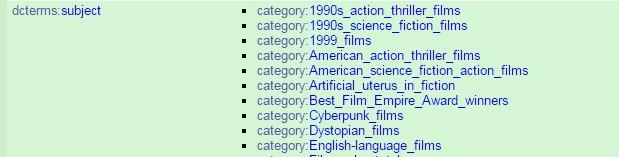
\includegraphics[width=\linewidth]{Images/Categories.jpg}
		\caption{Categories associated to the movie "The Matrix"}
		\label{fig:categories}
	\end{figure}
	
	Wikipedia categories are another important source of structure. Categories appear at the bottom of many Wikipedia pages and classify articles according to topics, domains, periods, places, genres, or other organizing principles. DBpedia represents these categories as resources and models their hierarchy using SKOS.\\
	
	A resource is linked to its categories through \texttt{dcterms:subject} (see figure \ref{fig:categories}). Category-to-category hierarchy is represented through \texttt{skos:broader}. The result is a graph of topical classification that can be traversed independently from the ontology class hierarchy.\\
	
	A simplified example is:
	
	\begin{lstlisting}
@prefix dbr:     <http://dbpedia.org/resource/> .
@prefix dbc:     <http://dbpedia.org/resource/Category:> .
@prefix dcterms: <http://purl.org/dc/terms/> .
@prefix skos:    <http://www.w3.org/2004/02/skos/core#> .
	
dbr:The_Matrix
  dcterms:subject dbc:Cyberpunk_films .
	
dbc:Cyberpunk_films
  skos:broader dbc:Science_fiction_films .
	\end{lstlisting}
	
	This representation deliberately uses SKOS rather than treating categories as ordinary ontology classes. A category is a conceptual indexing device: it groups resources according to topical relevance. The relation \texttt{skos:broader} expresses a broader topic, not necessarily a formal subclass relation. This distinction is important because category systems are often pragmatic and editorial, while ontology class hierarchies are expected to have more precise logical semantics.
	
	\subsection{Categories versus Ontology Classes}
	
	A DBpedia resource may be connected both to ontology classes and to categories. These two mechanisms serve different purposes. Ontology classes describe what kind of entity a resource is; categories describe topics under which the resource is classified. For example:
	
	\begin{lstlisting}
@prefix dbr:     <http://dbpedia.org/resource/> .
@prefix dbo:     <http://dbpedia.org/ontology/> .
@prefix dbc:     <http://dbpedia.org/resource/Category:> .
@prefix dcterms: <http://purl.org/dc/terms/> .

dbr:The_Matrix
  a dbo:Film ;
  dcterms:subject dbc:Cyberpunk_films .
	\end{lstlisting}
	
	The statement \texttt{a dbo:Film} assigns an ontology type. The statement using \texttt{dcterms:subject} assigns a topical category. Conflating the two would make the model less precise: being an instance of a class and being categorized under a topic are not the same modeling relation.
	
	\section{DBpedia as a Hub in the Linked Open Data Cloud}
	
	DBpedia has historically occupied a central position in the Linked Open Data cloud because it provides identifiers for a very large number of widely known entities. Datasets from different domains can use DBpedia URIs as external reference points. For example, a cultural heritage dataset, a geographic dataset, and a media dataset may all link to the same DBpedia resource when they describe the same city, person, organization, or creative work.\\
	
	This hub role is a direct consequence of Linked Data principles. A dataset does not need to copy DBpedia's information. It can publish its own local data and include links such as \texttt{owl:sameAs}, \texttt{skos:exactMatch}, \texttt{skos:closeMatch}, or domain-specific relations when appropriate. These links allow applications to discover additional descriptions and to merge contextual information from multiple sources.\\
	
	The choice of linking predicate depends on the strength of the intended relation. For identical real-world entities, an identity predicate may be appropriate. For concepts or classification terms, SKOS mapping properties may be safer because they distinguish exact matches from close but non-identical correspondences.
	
	\begin{lstlisting}
@prefix ex:   <http://example.org/resource/> .
@prefix dbr:  <http://dbpedia.org/resource/> .
@prefix owl:  <http://www.w3.org/2002/07/owl#> .
@prefix skos: <http://www.w3.org/2004/02/skos/core#> .
	
ex:localEntity123 owl:sameAs dbr:The_Matrix .
	
ex:localConcept456 skos:closeMatch dbr:Cyberpunk .
	\end{lstlisting}
	
	The first statement asserts identity between a local entity and a DBpedia resource. The second states a close conceptual match. The weaker SKOS relation is often preferable when linking thesauri, categories, keywords, or other conceptual resources, because conceptual equivalence is rarely as strict as entity identity.
	
	\section{Reuse of Existing Vocabularies}
	
	DBpedia also illustrates a general design principle for Linked Open Data: reuse established vocabularies whenever they express the intended meaning with sufficient precision. Reuse improves interoperability because the semantics of well-known terms is already shared by a community of publishers, consumers, and tools.\\
	
	In DBpedia, this principle appears in several places. Labels and comments use RDFS properties such as \texttt{rdfs:label} and \texttt{rdfs:comment}. Categories use SKOS relations such as \texttt{skos:broader}. Topic assignment uses Dublin Core Terms through \texttt{dcterms:subject}. Ontological descriptions use the DBpedia Ontology when more specific domain modeling is needed.\\
	
	A dataset publisher should follow the same approach. Before defining a new property or class, the publisher should check whether an existing vocabulary already covers the intended meaning. Reuse may be complete or partial. It is often reasonable to reuse standard terms for general aspects and introduce local terms only for concepts that are genuinely domain-specific.\\
	
	The following pattern is common:
	
	\begin{lstlisting}
@prefix ex:      <http://example.org/vocab/> .
@prefix dcterms: <http://purl.org/dc/terms/> .
@prefix skos:    <http://www.w3.org/2004/02/skos/core#> .

ex:LocalCategory
  a skos:Concept ;
  skos:prefLabel "Local category"@en ;
  skos:broader ex:BroaderLocalCategory .
	
ex:LocalDatasetRecord
  dcterms:subject ex:LocalCategory ;
  ex:domainSpecificProperty ex:DomainSpecificValue .
	\end{lstlisting}
	
	The example reuses SKOS for the category model and Dublin Core Terms for subject assignment, while reserving the local namespace \texttt{ex} for domain-specific information. This is preferable to redefining equivalents of \texttt{skos:Concept}, \texttt{skos:prefLabel}, or \texttt{dcterms:subject} without necessity.
	
	\subsection{When New Terms Are Necessary}
	
	Vocabulary reuse does not imply that new vocabularies should never be created. A new term is appropriate when existing vocabularies do not express the intended meaning, when the distinction is important for the application, or when the domain requires concepts that are not covered by general-purpose vocabularies.\\
	
	The key requirement is to introduce new terms deliberately. A local property should not duplicate an existing widely used property with the same meaning. Conversely, forcing an imprecise match to an existing term can damage data quality. Good modeling balances reuse and specificity: use common vocabularies for shared semantics, and extend them only where the domain requires additional precision.\\
	
	When extending a model, the relationship between local and external terms should be made explicit whenever possible. For example, a local class may be declared as a subclass of a more general external class, or a local property may be related to an external property when the semantics justifies it.
	
	\begin{lstlisting}
@prefix ex:   <http://example.org/vocab/> .
@prefix dbo:  <http://dbpedia.org/ontology/> .
@prefix rdfs: <http://www.w3.org/2000/01/rdf-schema#> .
	
ex:InteractiveFilm
  rdfs:subClassOf dbo:Film .
	
ex:interactionMechanism
  rdfs:domain ex:InteractiveFilm .
	\end{lstlisting}
	
	This type of extension preserves interoperability at the general level while allowing the local model to capture additional distinctions.
	
	\section{Practical Use of DBpedia in Applications}
	
	Applications commonly use DBpedia for enrichment, disambiguation, and navigation. A local dataset may contain an entity name as a string, such as the title of a work or the name of a person. Linking that string to a DBpedia URI turns it into a reference to a graph node with multilingual labels, types, categories, abstracts, and links to other datasets.\\
	
	This process is particularly useful when a local dataset has limited descriptive metadata. By linking to DBpedia, the dataset can support richer search and browsing. For example, a collection of films can be enriched with genres, directors, actors, categories, and multilingual labels. A collection of places can be connected to geographic, administrative, historical, and cultural descriptions. A collection of people can be enriched with affiliations, occupations, birthplaces, and related works, depending on the available data.\\
	
	The benefit is not automatic correctness. Entity linking must distinguish between homonyms, aliases, different editions, and resources with similar names. The presence of a DBpedia URI improves interoperability only when the link identifies the intended entity or concept accurately. For this reason, Linked Data publication should treat external links as part of the data quality process, not as an optional decoration.
	
	\section{Chapter summary}
	
	DBpedia transforms Wikipedia's semi-structured content into RDF and publishes it as Linked Open Data. Its resources are named by predictable URIs derived from Wikipedia article URLs, and their descriptions combine ontology-based facts, language-tagged labels, textual abstracts, categories, and links to other resources.\\
	
	The dataset demonstrates several central Linked Data practices: use dereferenceable URIs, distinguish literals from resource links, provide multilingual descriptions with language tags, model topic hierarchies through SKOS, and reuse established vocabularies such as RDFS, Dublin Core Terms, and SKOS when they capture the intended semantics. DBpedia is therefore both a major dataset in its own right and a practical model for designing interoperable Linked Data.
	
	\chapter{Mapping Relational Data to RDF}
	
	Relational databases and tabular datasets are frequent starting points for Linked Open Data publication. In the five-star model, tabular data published in a non-proprietary format already provides machine-processable information, but it does not yet expose entities as dereferenceable resources and does not express links through RDF predicates. The purpose of relational-to-RDF mapping is to transform rows, columns, keys, and relationships into RDF resources, properties, literals, and links.\\
	
	This transformation is relevant whenever a dataset must evolve from a merely machine-readable form to a machine-linkable form. The resulting RDF graph should preserve the information contained in the relational source while making entities addressable by URIs and relations explicit as RDF statements. In practice, this requires decisions about URI generation, class assignment, predicate naming, literal typing, treatment of null values, and representation of foreign keys.
	
	\section{Direct Mapping from Relational Data to RDF}
	
	A direct relational-to-RDF mapping translates the structure of a relational database into RDF using a systematic set of rules. Each table is treated as the source of a class of resources. Each row becomes an RDF resource. Each column becomes a predicate. Each cell value becomes the object of a triple, either as a literal or, when the value participates in a foreign-key relationship, as a link to another resource.\\
	
	The essential steps are the following:
	
	\begin{itemize}
	    \item generate a URI for each row, typically using the table name and the primary key value;
	    \item assign the generated resource to a class derived from the table name;
	    \item create one RDF statement for each non-null attribute value;
	    \item translate foreign-key relationships into URI links between the corresponding row resources.
	\end{itemize}
	
	Consider a relational database with two tables, \texttt{People} and \texttt{Addresses}. The table \texttt{People} contains an identifier, a name, and a reference to an address. The table \texttt{Addresses} contains an identifier, a city, and a state. The following fragment illustrates the relational source.
	
	\begin{lstlisting}
People
ID | fname | addr
7  | Bob   | 18
8  | Sue   | NULL

Addresses
ID | city      | state
18 | Cambridge | MA
	\end{lstlisting}
	
	A direct RDF representation can use the table name and primary key to build resource identifiers. The row \texttt{People(ID=7)} becomes the resource \texttt{<People/ID=7>}; the row \texttt{Addresses(ID=18)} becomes the resource \texttt{<Addresses/ID=18>}. The base URI provides the common namespace for the generated resources.\\
	
	The directive \texttt{@base} is part of the Turtle syntax and defines the base IRI against which relative IRIs are resolved. It does not create an RDF triple and it does not declare a resource; it only provides a common prefix used by the parser when expanding abbreviated IRIs written between angle brackets. In the example, the directive \texttt{@base <http://foo.example/DB/> .} means that an IRI such as \texttt{<People/ID=7>} is interpreted as \texttt{<http://foo.example/DB/People/ID=7>}. Similarly, \texttt{<Addresses/ID=18>} denotes \texttt{<http://foo.example/DB/Addresses/ID=18>}, while predicates such as \texttt{<People\#fname>} are expanded to\\
	\texttt{<http://foo.example/DB/People\#fname>}. The use of \texttt{@base} therefore keeps the mapping compact while preserving globally identifiable resources and properties.
	
	\begin{lstlisting}
@base <http://foo.example/DB/> .
@prefix xsd: <http://www.w3.org/2001/XMLSchema#> .
@prefix rdf: <http://www.w3.org/1999/02/22-rdf-syntax-ns#> .

<People/ID=7> rdf:type <People> .
<People/ID=7> <People#ID> 7 .
<People/ID=7> <People#fname> "Bob" .
<People/ID=7> <People#addr> 18 .
<People/ID=7> <People#ref-addr> <Addresses/ID=18> .

<People/ID=8> rdf:type <People> .
<People/ID=8> <People#ID> 8 .
<People/ID=8> <People#fname> "Sue" .
	
<Addresses/ID=18> rdf:type <Addresses> .
<Addresses/ID=18> <Addresses#ID> 18 .
<Addresses/ID=18> <Addresses#city> "Cambridge" .
<Addresses/ID=18> <Addresses#state> "MA" .
	\end{lstlisting}
	
	The triples preserve the content of the two tables while adding an RDF interpretation. The table \texttt{People} is represented as a class-like resource, and each person row is typed accordingly. The predicates \texttt{<People\#ID>}, \texttt{<People\#fname>}, and \texttt{<People\#addr>} correspond to columns. The predicate \texttt{<People\#ref-addr>} represents the foreign-key relationship from the person to the address resource.\\
	
	The distinction between \texttt{<People\#addr>} and \texttt{<People\#ref-addr>} is important. The former preserves the original column value as data; the latter expresses the relational link as an RDF link. The second form is the one that contributes directly to Linked Data navigation, because the object is a URI identifying another resource. The row for \texttt{Sue} has no address triple because the relational value is \texttt{NULL}; direct mappings normally omit triples for null values rather than representing null as a literal value.
	
	\section{Limits of Purely Automatic Direct Mapping}
	
	Direct mapping is useful because it provides a predictable translation from relational structures to RDF. It can be applied without designing a domain ontology in advance and without manually writing every triple. However, the resulting graph often mirrors the database schema too closely. Table names become class names, column names become predicate names, and internal database identifiers become part of public URIs.\\
	
	This behavior is acceptable for a mechanical export, but it is not always suitable for publication as high-quality Linked Open Data. Database schemas are usually designed for storage, integrity, and application efficiency, whereas RDF vocabularies should support interoperability and semantic reuse. A column name that is meaningful inside one database may be too local or ambiguous for external consumers. Similarly, a primary-key-based URI may be stable within a database but not necessarily meaningful or persistent as a public identifier.\\
	
	A further limitation is maintainability. If the database schema changes, a procedural conversion implementation must be updated accordingly. If the desired RDF output changes, for example because a different vocabulary must be reused, the conversion logic must again be modified. These issues motivated the adoption of declarative mapping languages, where the relationship between the relational source and the RDF target is expressed explicitly in a mapping document.
	
	\section{Declarative Mapping with R2RML}
	
	R2RML, the RDB to RDF Mapping Language, is a W3C language for describing customized mappings from relational databases to RDF graphs. Instead of hard-coding the conversion procedure, R2RML expresses how tables, columns, and relationships should be transformed into RDF resources and triples. An R2RML processor takes the relational database and the mapping document as input and produces the RDF graph as output.\\
	
	The central unit of an R2RML mapping is the \textbf{triples map}. A triples map specifies the logical table used as input, the subject map used to generate RDF subjects, and one or more predicate-object maps used to generate RDF properties and values. This makes the mapping declarative: the document states what RDF structure should be produced, while the processor handles the operational details of generating the triples.\\
	
	Consider a relational database containing an employee table and a department table.
	
	\begin{lstlisting}
EMP
EMPNO | ENAME | JOB   | DEPTNO
7369  | SMITH | CLERK | 10

DEPT
DEPTNO | DNAME     | LOC
10     | APPSERVER | NY
	\end{lstlisting}
	
	The column \texttt{EMP.DEPTNO} acts as a foreign key referencing \texttt{DEPT.DEPTNO}. In the RDF representation, this relational relationship should not be represented only as the literal value \texttt{10}; it should also become a link from the employee resource to the corresponding department resource. Thus, the employee identified by \texttt{EMPNO = 7369} can be represented as\\
	\texttt{<http://data.com/employee/7369>}, while the department identified by \texttt{DEPTNO = 10} can be represented as \texttt{<http://data.com/department/10>}.\\
	
	The mapping can be divided into two triples maps: one for employees and one for departments. The employee triples map generates employee resources, maps the employee attributes to RDF properties, and uses a referencing object map to generate the link to the corresponding department.
	
	\begin{lstlisting}
@prefix rr:  <http://www.w3.org/ns/r2rml#> .
@prefix ex:  <http://com/ns#> .
@prefix xsd: <http://www.w3.org/2001/XMLSchema#> .

<#EmployeeTriplesMap>
  rr:logicalTable [ rr:tableName "EMP" ];
		
rr:subjectMap [
  rr:template "http://data.com/employee/{EMPNO}";
  rr:class ex:Employee;
];
		
rr:predicateObjectMap [
  rr:predicate ex:employeeNumber;
  rr:objectMap [
    rr:column "EMPNO";
    rr:datatype xsd:integer;
  ];
];

rr:predicateObjectMap [
  rr:predicate ex:name;
  rr:objectMap [
    rr:column "ENAME";
    rr:datatype xsd:string;
  ];
];

rr:predicateObjectMap [
  rr:predicate ex:job;
  rr:objectMap [
    rr:column "JOB";
    rr:datatype xsd:string;
  ];
];

rr:predicateObjectMap [
  rr:predicate ex:departmentNumber;
  rr:objectMap [
    rr:column "DEPTNO";
    rr:datatype xsd:integer;
  ];
];

rr:predicateObjectMap [
  rr:predicate ex:department;
  rr:objectMap [
    rr:parentTriplesMap <#DepartmentTriplesMap>;
    rr:joinCondition [
      rr:child "DEPTNO";
      rr:parent "DEPTNO";
    ];
  ];
].
	\end{lstlisting}
	
	The first predicate-object maps expose the attributes of the employee row as RDF literals. The last predicate-object map is different: it does not take the object directly from a column value. Instead, it refers to another triples map through \texttt{rr:parentTriplesMap}. The join condition states that the value of \texttt{EMP.DEPTNO} must be matched with the value of \texttt{DEPT.DEPTNO}. Once the matching department row is found, the subject generated by \texttt{<\#DepartmentTriplesMap>} becomes the object of the property \texttt{ex:department}. For the employee \texttt{7369}, whose department number is \texttt{10}, this produces a link to \texttt{<http://data.com/department/10>}.\\
	
	The department triples map generates department resources. In addition to the attributes stored directly in the \texttt{DEPT} table, the example includes the number of employees belonging to each department. This value is not stored as a column in the table; it is derived by an SQL aggregation query.
	
	\begin{lstlisting}
<#DepartmentTriplesMap>
rr:logicalTable [
  rr:sqlQuery """
    SELECT
    DEPT.DEPTNO,
    DEPT.DNAME,
    DEPT.LOC,
    COUNT(EMP.EMPNO) AS STAFF
    FROM DEPT
    LEFT JOIN EMP
    ON DEPT.DEPTNO = EMP.DEPTNO
    GROUP BY
    DEPT.DEPTNO,
    DEPT.DNAME,
    DEPT.LOC
  """
];

rr:subjectMap [
  rr:template "http://data.com/department/{DEPTNO}";
  rr:class ex:Department;
];

rr:predicateObjectMap [
  rr:predicate ex:departmentNumber;
  rr:objectMap [
    rr:column "DEPTNO";
    rr:datatype xsd:integer;
  ];
];

rr:predicateObjectMap [
  rr:predicate ex:name;
  rr:objectMap [
    rr:column "DNAME";
    rr:datatype xsd:string;
  ];
];

rr:predicateObjectMap [
  rr:predicate ex:location;
  rr:objectMap [
    rr:column "LOC";
    rr:datatype xsd:string;
  ];
];

rr:predicateObjectMap [
  rr:predicate ex:staff;
  rr:objectMap [
    rr:column "STAFF";
    rr:datatype xsd:integer;
  ];
].
	\end{lstlisting}
	
	The derived attribute \texttt{STAFF} is computed by counting the employees associated with each department. The \texttt{LEFT JOIN} ensures that departments with no employees can still appear in the result, with a count equal to zero. The mapping then treats \texttt{STAFF} like any other column of the logical table produced by the SQL query.\\
	
	For the database instance shown above, the employee triples map generates the following RDF triples.
	
	\begin{lstlisting}
@prefix ex:  <http://com/ns#> .
@prefix rdf: <http://www.w3.org/1999/02/22-rdf-syntax-ns#> .
@prefix xsd: <http://www.w3.org/2001/XMLSchema#> .

<http://data.com/employee/7369>
  rdf:type ex:Employee ;
  ex:employeeNumber "7369"^^xsd:integer ;
  ex:name "SMITH" ;
  ex:job "CLERK" ;
  ex:departmentNumber "10"^^xsd:integer ;
  ex:department <http://data.com/department/10> .
	\end{lstlisting}
	
	The department triples map generates the following RDF triples.
	
	\begin{lstlisting}
<http://data.com/department/10>
  rdf:type ex:Department ;
  ex:departmentNumber "10"^^xsd:integer ;
  ex:name "APPSERVER" ;
  ex:location "NY" ;
  ex:staff "1"^^xsd:integer .
	\end{lstlisting}
	
	The triple \texttt{<http://data.com/employee/7369> ex:department <http://data.com/department/10>} is therefore produced by the foreign-key mapping, not by a simple column-to-literal transformation. Conversely, the triple \texttt{<http://data.com/department/10> ex:staff "1"\string^\string^xsd:integer} is produced from the derived column \texttt{STAFF} computed by the SQL query. This illustrates why R2RML is more expressive than a direct automatic mapping: it can generate RDF links from relational joins and can expose derived values computed at query level.
	
	\subsection{Subject Maps}
	
	A subject map defines how RDF subjects are generated from database rows. The most common mechanism is a URI template containing column references. In the employee example, the template
	
	\begin{lstlisting}
rr:template "http://data.com/employee/{EMPNO}"
	\end{lstlisting}
	
	generates one employee URI for each row in \texttt{EMP}. If the row has \texttt{EMPNO = 7369}, the resulting subject is \texttt{<http://data.com/employee/7369>}. The subject map may also assign a class, such as \texttt{ex:Employee}, to all resources generated by the triples map.\\
	
	This mechanism makes URI design explicit. Instead of accepting identifiers mechanically derived from internal table names, the publisher can define stable URI patterns aligned with the public dataset structure.
	
	\subsection{Predicate-Object Maps}
	
	A predicate-object map specifies which predicate is produced and how the corresponding object is obtained. For literal-valued properties, the object map can refer directly to a column. In the example, the value of \texttt{ENAME} becomes the object of the predicate \texttt{ex:name}.\\
	
	More complex mappings may generate objects through templates, constants, joins, or datatype specifications. The essential point is that the mapping file states the correspondence between relational data and RDF vocabulary terms. This allows the same source database to be republished under a different RDF model by changing the mapping rather than rewriting a conversion program.
	
	\section{Representing Relationships}
	
	Relational databases express relationships through keys. RDF expresses relationships through triples whose objects may be URIs. A correct relational-to-RDF mapping must therefore transform foreign-key references into links between generated resources.\\
	
	In a direct mapping, the foreign key from \texttt{People.addr} to \texttt{Addresses.ID} can be represented by a generated predicate such as \texttt{<People\#ref-addr>}. In a customized R2RML mapping, the same relationship can be mapped to a meaningful vocabulary property, for example \texttt{ex:department} in the employee-department case.\\
	
	The difference is not only syntactic. A generated predicate preserves the database structure, while a vocabulary predicate communicates the intended semantics of the relationship. For Linked Open Data publication, the second approach is usually preferable when an appropriate vocabulary exists or when a domain vocabulary has been designed for the dataset.
	
	\section{Advantages of Declarative Mappings}
	
	Declarative relational-to-RDF mapping provides several practical advantages over procedural conversion.
	
	\begin{itemize}
	    \item The intended RDF output is easier to inspect because the mapping document explicitly describes tables, subject templates, classes, predicates, and object sources.
	    \item The mapping is easier to maintain when the database schema changes or when the RDF publication model evolves.
	    \item The same relational source can be exported in different RDF shapes by modifying the mapping.
	    \item Existing vocabularies can be reused more systematically, improving interoperability with other datasets.
	    \item The mapping document can be treated as part of the dataset publication process, making the transformation more transparent and reproducible.
	\end{itemize}
	
	The main design task is to avoid treating RDF generation as a purely mechanical dump. A useful Linked Data publication should expose stable identifiers, use meaningful predicates, preserve relevant relational constraints as RDF links, and reuse shared vocabularies where possible. R2RML supports this task by making the transformation explicit and configurable while still allowing the conversion process to be automated.
	
	\chapter{Open Data Licensing}
	
	\section{Licensing as a Condition for Open Data}
	
	Publishing data on the Web does not automatically make it open. A dataset can be technically accessible, machine-readable, and even expressed in RDF, while still being legally unusable for redistribution, integration, or application development. Open Data therefore requires both a technical publication model and an explicit legal framework that defines what users are allowed to do with the data.\\
	
	In the five-star model of Linked Open Data, the first requirement is publication on the Web under an open license. This requirement is deliberately placed before machine readability, non-proprietary formats, RDF, and interlinking. Without a license that grants reuse rights, the technical quality of the dataset does not guarantee that third parties can legally copy it, combine it with other datasets, or publish derived resources.\\
	
	A license for open data should clarify at least the following aspects:
	
	\begin{itemize}
	    \item whether the dataset may be copied and redistributed;
	    \item whether it may be modified, transformed, or combined with other data;
	    \item whether it may be used for commercial purposes;
	    \item whether derivative works must preserve the same license;
	    \item whether attribution to the original source is required;
	    \item whether there are restrictions on the creation of derivative works.
	\end{itemize}
	
	These conditions are not only legal details. They directly affect interoperability. A dataset with a restrictive license may be technically linkable, but unsuitable for integration into applications, knowledge graphs, or derived datasets whose licensing requirements are incompatible. Conversely, a permissive license facilitates reuse, enrichment, and redistribution, which are essential properties of a functioning Linked Open Data ecosystem.
	
	\section{Creative Commons Licenses}
	
	Creative Commons licenses provide a family of standardized licenses used to express permissions and restrictions for creative works and, in many contexts, for datasets. Their modular structure makes them useful for describing different degrees of openness. The conditions can be combined to indicate whether attribution is required, whether commercial use is allowed, whether derivative works are permitted, and whether derivatives must be shared under compatible terms.
	
	\subsection{Attribution}
	
	\begin{figure}[!h]
		\centering
		
\includegraphics[width=0.1\linewidth]{Images/CC-BY.png}
		\caption{CC-BY icon}
		\label{fig:cc_by}
	\end{figure}
	
	The attribution condition, usually abbreviated as \texttt{BY} and indicated using the icon in figure \ref{fig:cc_by}, requires users to give appropriate credit to the original author or publisher. In the context of data, attribution normally means citing the source of the dataset and, when relevant, indicating whether modifications have been made.\\
	
	The \texttt{CC-BY} license allows copying, redistribution, remixing, transformation, and reuse for any purpose, including commercial purposes, provided that attribution is given. For open datasets, this is a relatively permissive model because it allows both direct reuse and the production of derived datasets or applications. Its main obligation is informational rather than restrictive: users must preserve a clear reference to the origin of the data.
	
	\subsection{Non-Commercial Use}
	
	\begin{figure}[!h]
		\centering
		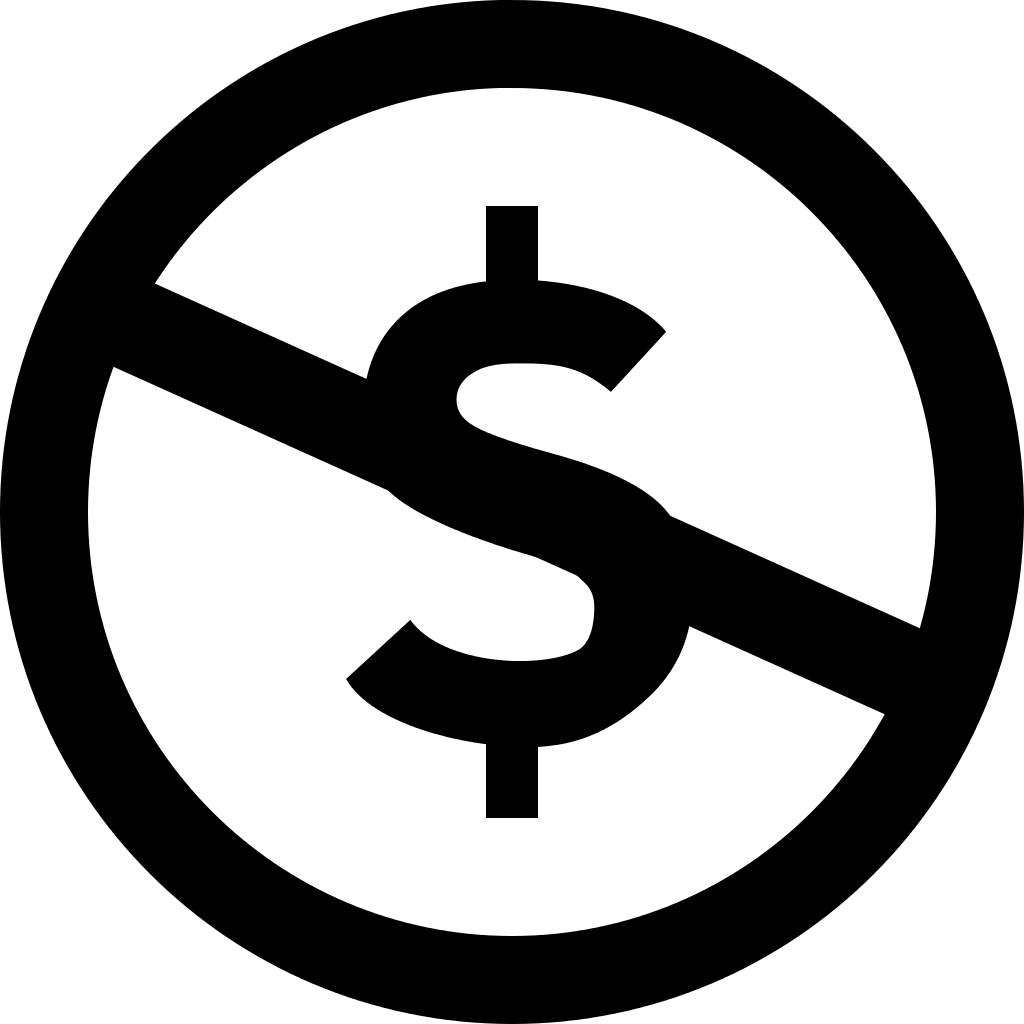
\includegraphics[width=0.1\linewidth]{Images/CC-NC.png}
		\caption{CC-NC icon}
		\label{fig:cc_nc}
	\end{figure}
	
	The non-commercial condition, abbreviated as \texttt{NC} and indicated using the icon in figure \ref{fig:cc_nc}, permits copying, distribution, display, execution, and derivative works only for non-commercial purposes. In practice, this condition restricts reuse by companies, commercial platforms, and applications whose business model involves monetization.\\
	
	For Linked Open Data, \texttt{NC} restrictions can reduce integrability. A dataset licensed only for non-commercial use may be unsuitable for mixed ecosystems where public, academic, and private actors contribute to the same knowledge graph. Even when the technical representation is fully interoperable, the legal condition can prevent some forms of downstream use.
	
	\subsection{No Derivative Works}
	
	\begin{figure}
		\centering
		
\includegraphics[width=0.1\linewidth]{Images/CC-ND.png}
		\caption{CC-ND icon}
		\label{fig:cc_nd}
	\end{figure}
	
	The no-derivatives condition, abbreviated as \texttt{ND} and indicated using the icon in figure \ref{fig:cc_nd}, permits redistribution of unchanged copies but does not allow derivative works. Applied to datasets, this condition is particularly limiting because many useful data operations can be considered transformative: cleaning, normalization, schema mapping, enrichment, linkage, aggregation, and conversion into RDF may all produce a derived dataset.\\
	
	A dataset under a no-derivatives condition may still be consultable and redistributable in its original form, but it is poorly aligned with the goals of Linked Open Data. Linked Data publication often requires transformation, entity reconciliation, vocabulary mapping, and the addition of links to external resources. These operations are central to the creation of four-star and five-star datasets, and they require permission to produce modified or enriched versions.
	
	\subsection{Share Alike}
	
	\begin{figure}[!h]
		\centering
		
\includegraphics[width=0.1\linewidth]{Images/CC-SA.png}
		\caption{CC-SA icon}
		\label{fig:cc_sa}
	\end{figure}
	
	The share-alike condition, abbreviated as \texttt{SA} and indicated using the icon in figure \ref{fig:cc_sa}, allows derivative works but requires them to be distributed under the same license or under a compatible license. This condition is intended to preserve openness across derivative works. If a dataset is reused and extended, the resulting dataset must remain available under equivalent terms.\\
	
	In data ecosystems, share-alike conditions can support the construction of a common open resource pool, but they also introduce compatibility issues. When data from multiple sources are combined, their licenses must be mutually compatible. If two datasets impose different share-alike obligations, publishing a single derived dataset may become legally complex or impossible without additional permissions.
	
	\subsection{No Rights Reserved}
	
	\begin{figure}
		\centering
		
\includegraphics[width=0.1\linewidth]{Images/CC0.png}
		\caption{CC0 icon}
		\label{fig:cc0}
	\end{figure}
	
	The \texttt{CC0} public-domain dedication is the most permissive Creative Commons instrument. It allows copying, modification, distribution, and use, including commercial use, without requesting permission and without imposing attribution as a legal obligation. It is indicated using the icon in figure \ref{fig:cc0}.\\
	
	For open data publication, \texttt{CC0} maximizes reuse because it removes the main legal constraints on transformation and redistribution. It is especially suitable when the publisher wants to encourage broad reuse, integration into third-party services, and incorporation into derived knowledge graphs. Although attribution may still be considered good scholarly or institutional practice, \texttt{CC0} does not make it a licensing requirement.
	
	\section{Licensing Conditions and Data Reuse}
	
	The main Creative Commons conditions can be understood as constraints on different dimensions of reuse.
	
	\begin{itemize}
	    \item \texttt{BY} constrains attribution, but allows broad reuse.
	    \item \texttt{NC} constrains the economic context of reuse.
	    \item \texttt{ND} constrains transformation and derivation.
	    \item \texttt{SA} constrains the license of derivative works.
	    \item \texttt{CC0} removes most reuse constraints.
	\end{itemize}
	
	For Linked Open Data, the most relevant question is not only whether the data can be accessed, but whether it can be processed, transformed, linked, republished, and used in applications. Licenses that allow modification and redistribution are therefore better aligned with the Linked Data workflow. Licenses that prohibit derivative works are generally problematic, while non-commercial and share-alike restrictions must be evaluated with respect to the expected reuse scenario.\\
	
	This evaluation is particularly important when data are used to produce a derived RDF dataset. The conversion of a tabular dataset into RDF may involve changes in identifiers, data model, vocabulary, and links to external resources. The resulting graph may be structurally different from the original dataset, even when it preserves the original informational content. A suitable license must therefore permit the creation and publication of such derived representations.
	
	\section{Public Sector Open Data}
	
	Open data policies are especially relevant in the public sector because public administrations produce datasets with high social, institutional, and economic value. Examples include geographic data, legislative data, statistical data, administrative registers, transportation data, cultural heritage data, and public spending data. Making these datasets available under open licenses allows citizens, researchers, companies, and other administrations to inspect, combine, and reuse information that would otherwise remain fragmented.\\
	
	In public-sector contexts, open data licensing supports several goals:
	
	\begin{itemize}
	    \item transparency, because public information can be inspected and redistributed;
	    \item accountability, because data can be independently analyzed;
	    \item administrative interoperability, because different offices and institutions can reuse each other's datasets;
	    \item service development, because applications can be built on public data sources;
	    \item data enrichment, because third parties can link public data to other open datasets.
	\end{itemize}
	
	The availability of public data is therefore not only a publication requirement, but also a basis for data-driven services and knowledge infrastructures. The Linked Open Data approach strengthens this objective by encouraging public datasets to use stable identifiers, RDF vocabularies, and links to other datasets.
	
	\section{Italian Open Data License}
	
	The Italian Open Data License is a licensing framework designed for the sharing and reuse of public-sector data in Italy. It reflects the broader principle that public data should be available for reuse and that public administrations should publish data in a form compatible with access, redistribution, and application development.\\
	
	The license grants permissions that are essential for open data reuse. Users may browse, extract, download, copy, publish, redistribute, and transmit data. They may also create derivative works, for example by combining the data with other information sources, and may develop applications that use public data sources.\\
	
	These permissions are aligned with the typical lifecycle of open public data:
	
	\begin{enumerate}
	    \item a public administration publishes a dataset;
	    \item users retrieve and inspect the data;
	    \item developers or data publishers transform the data into formats suitable for processing;
	    \item the data are combined with other sources or enriched with additional links;
	    \item applications, analyses, or derived datasets are published.
	\end{enumerate}
	
	The license therefore supports not only passive access, but active reuse. This distinction is central for Linked Open Data, where a dataset becomes more valuable when it can be transformed, linked, and integrated into larger graphs.
	
	\subsection{IODL 1.0}
	
	The first version of the Italian Open Data License allowed broad reuse of public data, including extraction, redistribution, derivative works, and application development. Its distinctive constraint was a share-alike obligation: derivative works and applications based on the licensed data had to preserve the same license.\\
	
	This condition ensured that reuse remained open, but it also introduced compatibility constraints. When data licensed under a share-alike obligation are combined with data under different licensing terms, the resulting work must satisfy all applicable requirements. This can complicate integration when several datasets are merged into one derived product.
	
	\subsection{IODL 2.0}
	
	The second version simplified the reuse model. Instead of requiring derivative works and applications to preserve the same license, it requires the licensee to cite the source of the information. This makes the license closer to an attribution-based model and reduces the legal friction associated with combining public data with other datasets.\\
	
	For Linked Open Data publication, this change is significant. Attribution requirements are usually easier to satisfy in RDF datasets, metadata records, and application documentation than share-alike obligations. A dataset derived from multiple sources can include provenance and attribution metadata while still being distributed under a license compatible with the overall project.
	
	\section{Licensing Metadata in Linked Data}
	
	Licensing information should be part of the metadata associated with a dataset. A Linked Data publisher should not rely only on a human-readable web page that describes the license. The dataset itself should contain machine-processable metadata indicating the applicable rights and license conditions.\\
	
	Dublin Core properties are commonly used for this purpose. A dataset can include rights information, a license reference, publisher metadata, and source attribution. These metadata do not replace the legal text of the license, but they make licensing information discoverable and reusable by software agents, catalogues, and data integration pipelines.\\
	
	At the dataset level, licensing metadata should identify:
	
	\begin{itemize}
	    \item the license applied to the dataset;
	    \item the publisher or rights holder;
	    \item the attribution text or citation requirement;
	    \item the date or version of the dataset;
	    \item relevant provenance information when the dataset is derived from other sources.
	\end{itemize}
	
	At the resource level, additional rights information may be necessary when a dataset aggregates content with heterogeneous legal conditions. In such cases, the publisher should avoid implying that the same license applies uniformly to all resources unless this has been verified.
	
	\section{Choosing a License for Linked Open Data}
	
	The choice of license should be guided by the intended reuse scenario. A dataset meant to maximize dissemination and integration should use a permissive license such as \texttt{CC0} or an attribution-based license. A dataset whose publisher wants to preserve recognition should use an attribution requirement. A dataset whose publisher wants derivatives to remain open may use a share-alike condition, while accepting the corresponding compatibility costs.\\
	
	For Linked Open Data, licenses should be evaluated according to the operations that the publisher expects users to perform:
	
	\begin{itemize}
	    \item conversion into RDF or other machine-processable formats;
	    \item vocabulary mapping and schema alignment;
	    \item entity reconciliation and linking to external datasets;
	    \item enrichment with additional statements;
	    \item redistribution through catalogues, dumps, APIs, or SPARQL endpoints;
	    \item incorporation into applications and analytical workflows.
	\end{itemize}
	
	A license that prevents or complicates these operations weakens the practical openness of the dataset. The strongest Linked Open Data publications combine technical interoperability with explicit legal permissions for reuse, transformation, interlinking, and redistribution.

\end{document}